\subsection{Electrostatics}

\subsubsection{Conducting ball}\label{Conducting ball}
We have a conducting ball which is placed in an homogenous electric field $\vec{E}=E_{z}\hat{z}$. The starting point is to consider the general spherical solution for a "hollow" sphere on a constant field. Let's discuss this in depth.

This sphere has charge that is homogeneously distributed.  On top of that, we can infer the following: If the field $\vec{E}$ is constant, the potential of this field should be linear with respect to $z$, as $-\vec{\nabla} \Phi= \vec{E}$. So $V \sim E_{0} z \: \hat{z}$.  But this would only be if the sphere was not present there. We also have to account for the field generated by the charge of the sphere and, hence, the potential of it. But here comes the trick. The potential generated by the sphere in negligible from far away. Why? We know that $\vec{E}=0$ inside conductors, so the potential $\Phi$ inside of  the sphere is a constant. By Gauss, we also know that the electric field generated by the sphere outside decreases proportionally as $\vec{E} \propto \tfrac{Q}{r^{2}}$.  When $r \gg R$, with $r$ being the observation position, we have that $\vec{E} \sim 0$.

So we know how the potential $\Phi$ (hence $\vec{E}$) looks like at two specific regimes. On the surface of the sphere this is:

\begin{equation}
	\Phi_{r=R} = -\frac{Q}{4 \pi \epsilon_{0} R},
\end{equation}

and far far away from it, which goes as:

\begin{equation}
	\Phi_{r\gg R} = \Phi_{\text{field}} + \Phi_{\text{sphere}} = E_{0} \underbrace{r \cos \theta}_{z} - \cancel{\frac{Q}{4 \pi \epsilon_{0} R}}.
\end{equation}

How does $\vec{E}$ look like in some mid region? Again, if we know the potential, we know the field. We have seen what the most general solution for the Laplace equation with azimuthal symmetry is given by:

\begin{equation}
	\Phi (r, \theta) = \sum_{\ell=0}^{} \left(A_{\ell} r^{\ell} + \frac{B_{\ell}}{r^{\ell+1}}\right) P_{\ell} (\cos \theta).
\end{equation}

Where $P_{\ell}(\cos \theta)$ are Legendre polynomials... If we expand the first few terms of previous expression we can see that:

\begin{equation}
	\Phi(r,\theta) = \underbrace{\left(A_{0} + \tfrac{B_{0}}{r}\right)}_{f_{0}(r)} \underbrace{P_{0}}_{1} + \underbrace{\left(A_{1} r  + \tfrac{B_{1}}{r^{2}}\right)}_{f_{1}(r)} \underbrace{P_{1}}_{\cos \theta} + \cdots
\end{equation}

it looks quite similar to the given Ansatz in the statement of the problem! In fact, we can now use this expression to fix the values of the coefficients $A_{\ell}, B_{\ell}$ with help of boundary conditions $\Phi_{r= R}$ and $\Phi_{r \gg R}$.

\begin{align}\label{finalfixing}
	\begin{split}
		\Phi_{r = R} &=   -\tfrac{Q}{4 \pi \epsilon_{0} R} = \left(A_{0} + \tfrac{B_{0}}{R}\right) + \left(A_{1} r  + \tfrac{B_{1}}{R^{2}}\right) \cos \theta =\\
		&= \cdots \text{matching powers of $R$}\cdots =\\
		&\rightarrow B_{0} = -\tfrac{Q}{4 \pi \epsilon_{0}},\\
		&\rightarrow  A_{0} +  \left(A_{1} r  + \tfrac{B_{1}}{R^{2}}\right) \cos \theta = 0.
	\end{split}
\end{align}

If we use the boundary condition at $\infty$, we obtain that:

\begin{align}
	\begin{split}
		\Phi_{r \rightarrow \infty} &=   -E_{0} r \cos \theta = A_{0} + \cancel{\tfrac{B_{0}}{r}} + \left(A_{1} r + \cancel{\tfrac{B_{1}}{r^{2}}} \right)\cos \theta =\\
		&= \cdots \text{matching powers of $r$}\cdots =\\
		&\rightarrow A_{1} = -E_{0},\\
		&\rightarrow  A_{0}  = 0.
	\end{split}
\end{align}

We only need to fix the value of $B_{1}$. With all previous values fixed, go back to equation \ref{finalfixing} to see obtain:

\begin{equation}
	B_{1} = E_{0} R^{3}.
\end{equation}

Then, all values together yield the following result:

\begin{equation}
	\Phi(r,\theta) = - \tfrac{Q}{4 \pi \epsilon_{0} r} - E_{0} R \cos \theta \left(\tfrac{r}{R} - \tfrac{R^{2}}{r^{2}}\right),
\end{equation}

which one can easily see that behave as expected when $r\rightarrow 0$ and $r =R$. The only remaining thing is to compute the value of the electric field $\vec{E}$ given this potential. As we are dealing with an azimuthal symmetry, the gradient should be used in spherical coordinates.  Then:

\begin{equation}
	\vec{E} = -\left(\tfrac{Q}{4 \pi \epsilon_{0} r} + E_{0} R \cos \theta \left(\tfrac{1}{R} + \tfrac{2R^{2}}{r^{3}}\right)\right) \hat{r} + \sin \theta E_{0} R \left(\tfrac{1}{R} - \tfrac{R^{2}}{r^{3}}\right) \hat{\theta}.
\end{equation}

\subsubsection{Conducting ball Again}\label{Conducting ball Again}
Let start by noting that the method of images consist of creating a fake charge $q_{f}$ such that we can reproduce the result of the original set up in an easier way. In this specific case, as we have the sphere earthed, we already know that the potential $\phi$ on its surface is equal to 0 ($\phi(R)$ =0). Several points to consider in the current set up:

\begin{enumerate}
	\item The charge $q_{t}$ (t for true) can be located \textbf{anywhere} inside the sphere. The important thing is that the sphere is earthed.
	\item As we have axial symmetry, this problem can be reduced to a two dimensional problem. We can use polar coordinates.
\end{enumerate}

A rough sketch of this set-up considering a mirror images can be found in fig(\ref{fig:Charge}).

\begin{figure}[h!]
	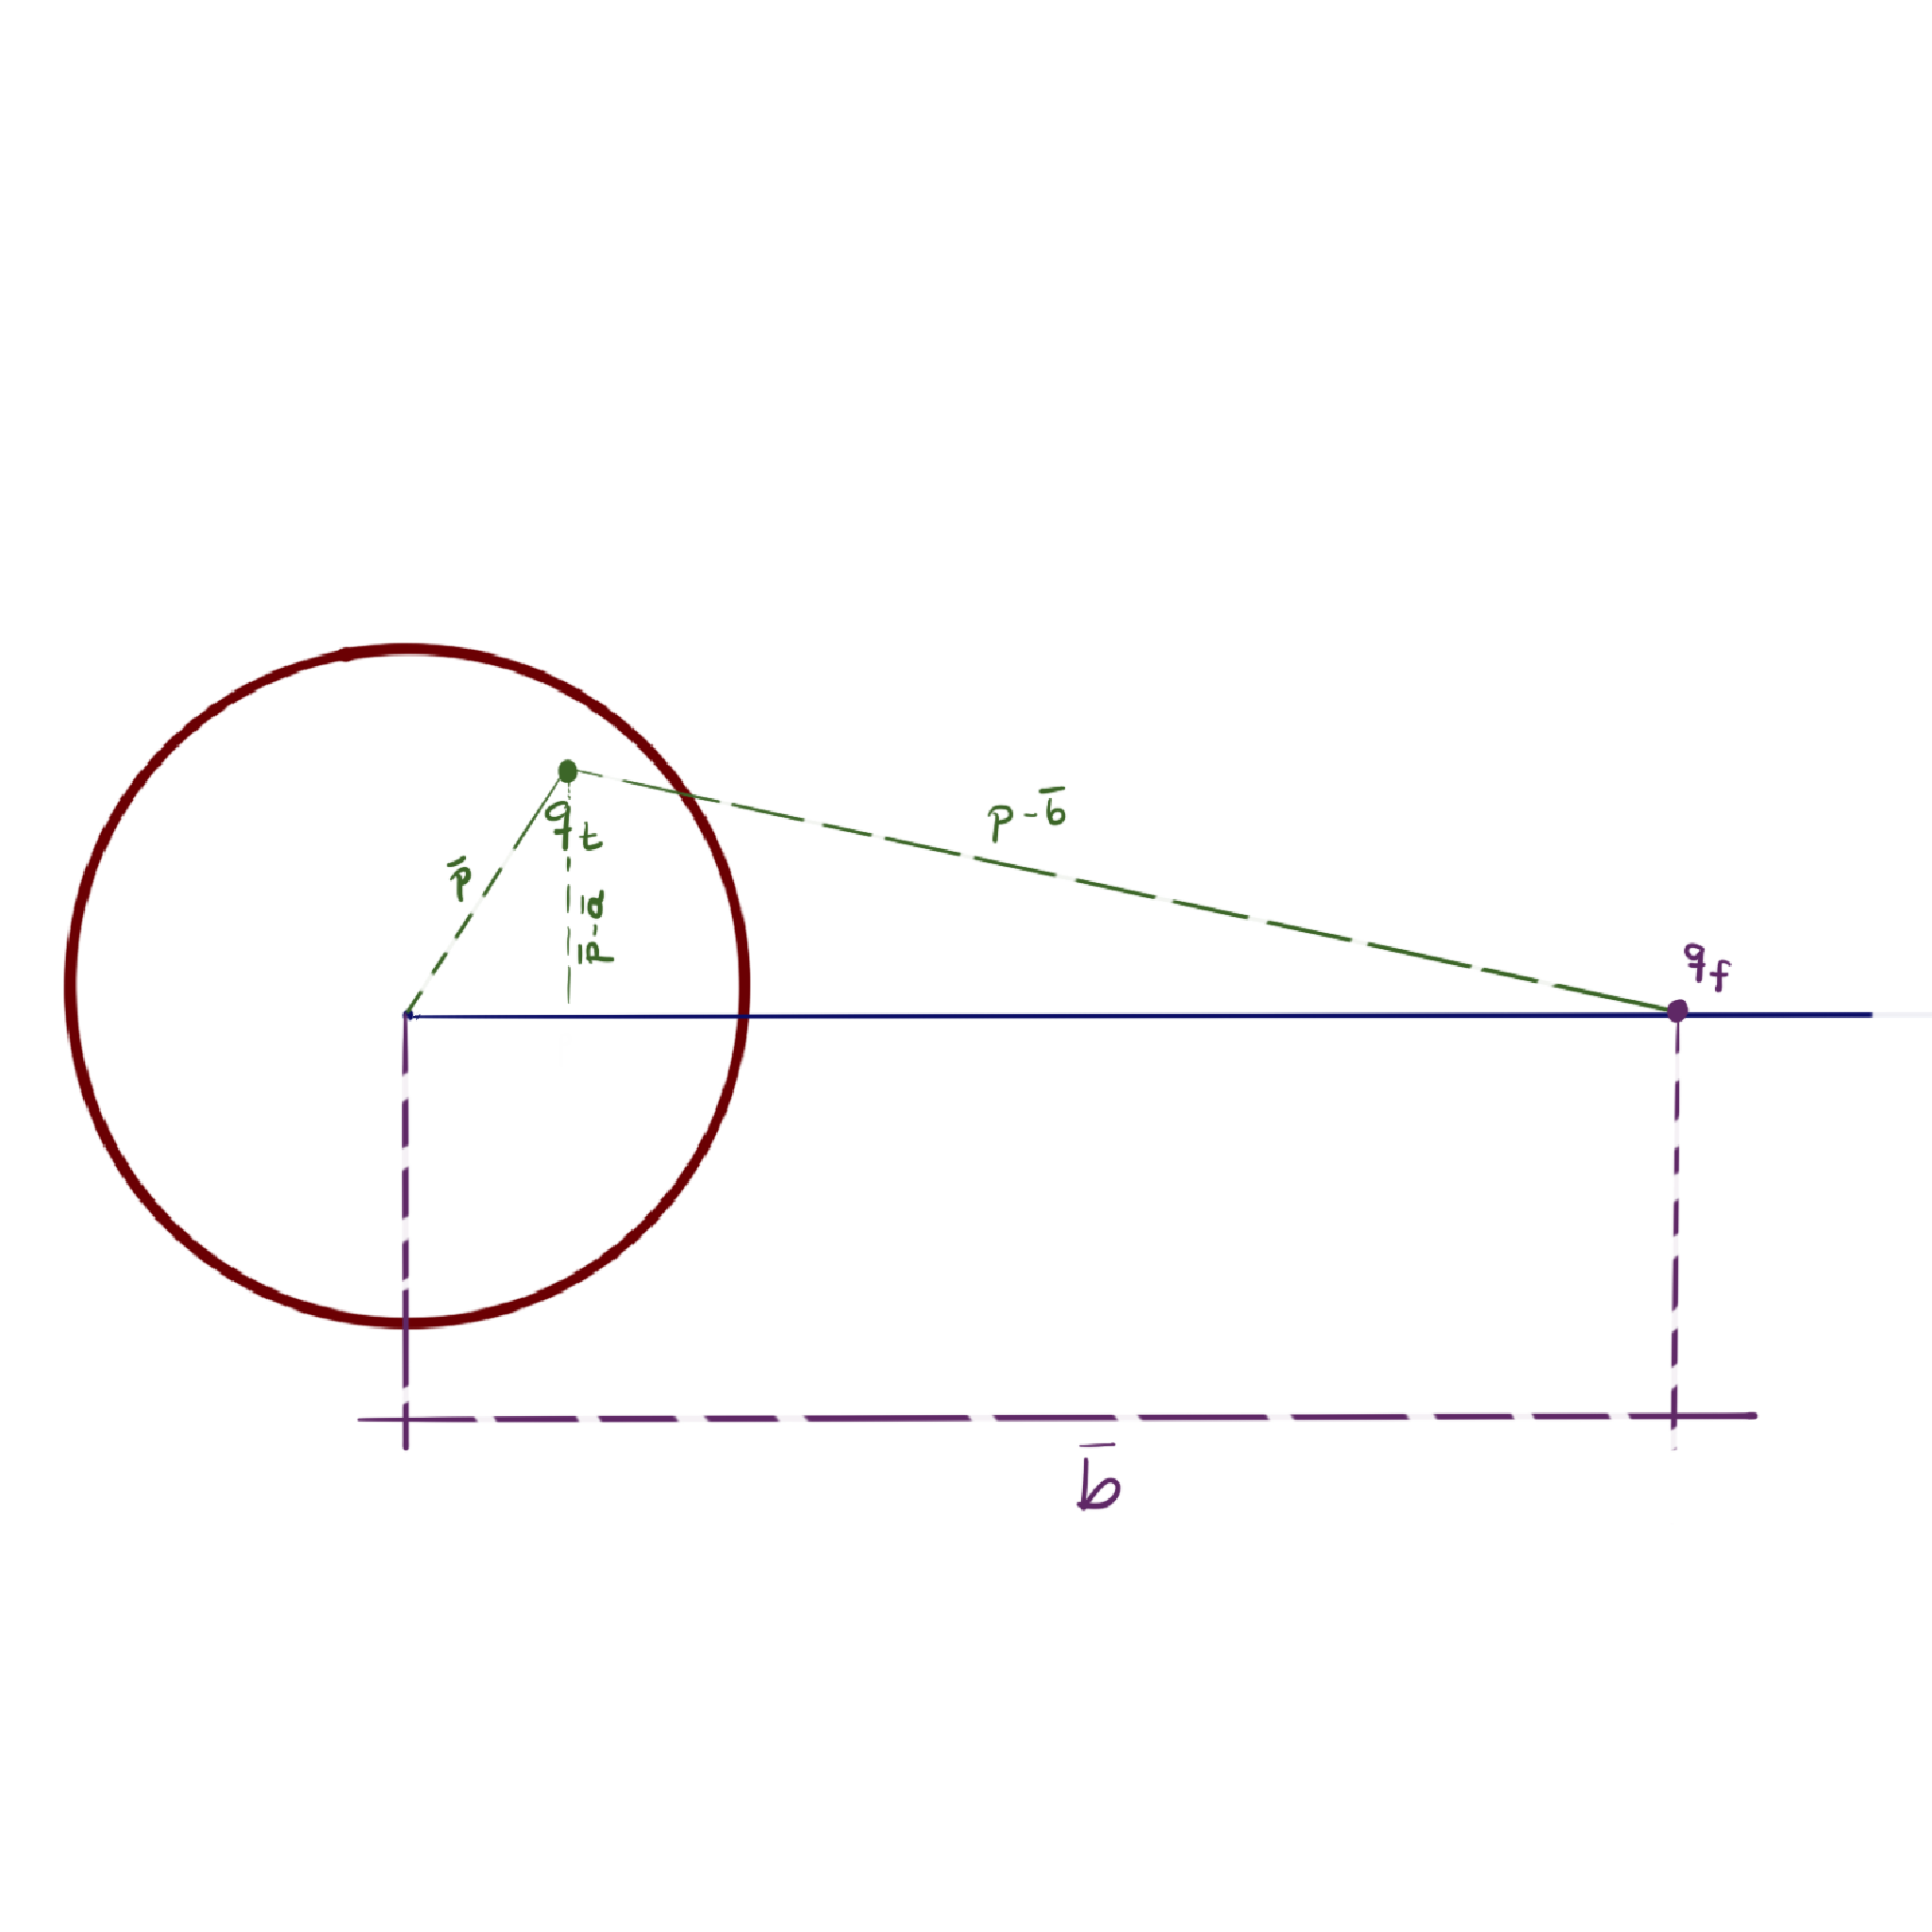
\includegraphics[width=9cm]{figures/MirrorCharge.png}
	\centering
	\caption{A rough sketch of this system studied by the method of images.}
	\label{fig:Charge}
\end{figure}

Then, the potential of this two charges, is given by superposition as:

\begin{equation}
	\phi (\vec{r}) = \frac{1}{4\pi \epsilon_{0}}\left(\frac{q_{t}}{\left|\vec{r}_{t}\right|} + \frac{q_{f}}{\left|\vec{r}_{f}\right|}\right),
\end{equation}

where $q_{f}$ stands for false charge/mirror charge. Imposing the boundary condition on the surface $\phi =0$, we have:

\begin{equation}
	\frac{q_{t}}{\left|\vec{p}-\vec{a}\right|} = \frac{-q_{f}}{\left|\vec{p}-\vec{b}\right|}.
\end{equation}

Now, we have to realise that we have two potential positions $(a,b)$ to fix, but just one equations... This issue can be easily solved by accounting for two possible set ups:

\begin{enumerate}
	\item Case where $p_{x} = R, p_{y}= 0$.
	In this case we will arrive to an equation that looks like:

	\begin{equation}\label{firstcase}
		\frac{q_{t}}{\left|R-a\right|} = \frac{-q_{f}}{\left|R-\vec{b}\right|} \rightarrow -\frac{q_{t}}{q_{f}} = \frac{R-a}{R-b}.
	\end{equation}

	Which is a good candidate as equation to solve for one of the variables. The other can be obtained by:

	\item Case where $p_{x} = 0, p_{y}= R$.
	
	This will give another equation as:

	\begin{equation}\label{secondcase}
		-\frac{q_{t}}{q_{f}} = \sqrt{\frac{R^{2}+a^{2}}{R^{2}+b^{2}}},
	\end{equation}

	which one can square both sides to get rid of the root.
\end{enumerate}

From these two set-ups, one should realise that LHS of equations (\ref{firstcase},\ref{secondcase}) are the same. Hence, equate them and manipulate the algebra to arrive to:

\begin{equation}
	\left(R^{2}+a^{2}\right)\: b - a \: b^{2} = R^{2} a.
\end{equation}

This is a well-known second order equation that gives two solutions for $b$ as: $b_{1} = a$, which makes no sense, as it tells us to place both charges at the same position, and $b_{2} = \tfrac{R^{2}}{a}$, which relates $a$ and $b$ in a non-trivial way. Introduce this result into any of both previous cases (\ref{firstcase}, \ref{secondcase}) to find the relation between the charges expressed as:

\begin{equation}
	q_{f} = - \frac{R \: q_{t}}{a}
\end{equation}

With this result the potential $\phi$ follows as:


\begin{align}
		\phi (\vec{r}) &= \frac{1}{4\pi \epsilon_{0}}\left(\frac{q_{t}}{\left|\vec{p}-\vec{a}\right|} - \frac{q_{t} \tfrac{R}{a}}{\left|\vec{p}- \left(\tfrac{R^{2}}{a},0\right)\right|}\right)=\\
		&=\frac{q_{t}}{4\pi \epsilon_{0}}\left(\frac{1}{\sqrt{r^{2}+a^{2}-2r a \cos \theta}} - \frac{1}{\tfrac{a}{R}\sqrt{r^{2}+\tfrac{R^{4}}{a^{2}}-2r \tfrac{R^{2}}{a} \cos \theta}}\right).
\end{align}


The electric field $\vec{E}$ follows from taking the minus gradient of previous expression. To obtain the induced charge density, we just need to recall that it is given the derivative of the potential $\phi$ respect to the normal of the surface where we want to evaluate such density, i.e.

\begin{equation}
	\sigma = - \epsilon \frac{\partial \phi}{\partial \vec{n}},
\end{equation}
In our case, due to spherical sym $\vec{n} = r$ and the surface of the sphere lies on $r=R$, so we just have to evaluate there. If one is careful with all the arithmetic and simplify cautiously,  the result is:

\begin{equation}
	\sigma = \frac{-q \: \epsilon}{4 \pi \epsilon_{0} a R} \left(\frac{1-\tfrac{R^{2}}{a^{2}}}{\sqrt[3]{\tfrac{R^{2}}{a^{2}} +1 - 2 \tfrac{R}{a}\cos \theta}}\right).
\end{equation}

Regarding the Gauss theorem for the electric field outside the sphere, it will the total charge inside the sphere divided by the total area where we evaluate the field. 

Solutions b and c for this problems follows exactly the same steps as we have previously done. The main difference can be found in the boundary condition on the surface of the sphere. As this is not any longer connected to earth, the potential on the surface will be given by:

\begin{equation}
	\phi (R) = V_{0}.
\end{equation}

In any case, one can repeat both cases for different positions of the inner charge to extract that the new fake charge $q_{f}'$ is:

\begin{equation}
	q_{f}' = q_{f} + V_{0}.
\end{equation}

From that point on, the rest of the exercise is straightforward to adapt to this new BC.

\subsubsection{The Capacitance of an off-centered Capacitor}\label{The Capacitance of an off-centered Capacitor}

Given the description of the statement, the first thing should be to draw something similar to this sketch:

\begin{figure}[h]
	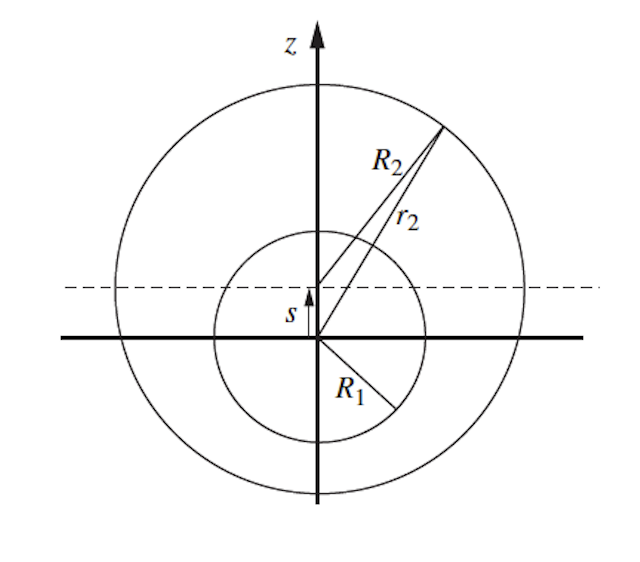
\includegraphics[width=8cm]{figures/capacitoroff.png}
	\centering
	\caption{A rough sketch of the system we want to study....}
\end{figure}

\textbf{1):}

Let $\left(r_{2}, \theta\right)$ denote a point on the outer shell with respect to the origin of the inner shell (The small one). By the law of cosines, the difference between $R_{2}^{2}$ (big capacitor centre) and $r^{2}$ (small centre) is given by: $R_{2}^{2}=r_{2}^{2}+s^{2}-2 r_{2} s \cos \theta$. Therefore, expanding the square root of $r_{2}$ to first order in $s$, the boundary of the outer shell is:
	
\begin{equation}
	r_{2}=R_{2}+s \cos \theta.
\end{equation}

If the shells were exactly concentric, the potential between them would have the form $\varphi(r)=a+b / r$. Therefore, in light of the expansion to first order and the general solution of Laplace's equation in polar coordinates, we expect the potential in the space between the displaced shells to take the form\footnote{This is an Ansatz of the Laplace equation. Observe that the first term is the zeroth order in the expansion in terms of Legendre polynomials for the most general solution, and the second term, is the subleading order, but, there is an "s" in front of everything. This is considered as a perturbation, as the inner sphere is slightly out of the centre.}:

\begin{equation}\label{potentialexpression}
	\varphi(r, \theta)=a+\frac{b}{r}+s\left(c r+\frac{d}{r^{2}}\right) \cos \theta+O\left(s^{2}\right)
\end{equation}

To order $s$, fixing the boundary conditions at the shell surfaces we get
\begin{equation}
	\begin{split}\label{boundarycon}
		V_{1}&=\varphi\left(R_{1}, \theta\right)=a+\frac{b}{R_{1}}+s\left(c R_{1}+\frac{d}{R_{1}^{2}}\right) \cos \theta,\\
		V_{2}&=\varphi\left(r_{2}, \theta\right) =a+\frac{b}{R_{2}+s \cos \theta}+s\left(c\left[R_{2}+s \cos \theta\right]+\frac{d}{\left[R_{2}+s \cos \theta\right]^{2}}\right) \cos \theta= \\
		&=a+\frac{b}{R_{2}}+s\left(c R_{2}+\frac{d}{R_{2}^{2}}-\frac{b}{R_{2}^{2}}\right) \cos \theta.
	\end{split}
\end{equation}

We know that the potential on the BC $V_{1}$ and $V_{2}$ are constants, so the coefficients of $\cos \theta$ must vanish in (\ref{boundarycon}). This fixes $d=-c R_{1}^{3}$ and $b=c\left(R_{2}^{3}-R_{1}^{3}\right) .$ Moreover, subtracting both conditions in (\ref{boundarycon}) we get an extra equation as:

\begin{equation}
	b=\left(V_{1}-V_{2}\right) R_{1} R_{2} /\left(R_{2}-R_{1}\right).
\end{equation}

so $c$ and $d$ written in terms of $R_{i}$ are:

\begin{equation}
	c=\left(V_{1}-V_{2}\right) \frac{R_{1} R_{2}}{\left(R_{2}^{3}-R_{1}^{3}\right)\left(R_{2}-R_{1}\right)}, \quad \quad d=-\left(V_{1}-V_{2}\right) \frac{R_{1}^{4} R_{2}}{\left(R_{2}^{3}-R_{1}^{3}\right)\left(R_{2}-R_{1}\right)}.
\end{equation}

Using (\ref{potentialexpression}), we can determine that the charge density on the surface of the inner shell is:

\begin{equation}
	\sigma(\theta)=-\left.\epsilon_{0} \frac{\partial \varphi}{\partial r}\right|_{r=R_{1}}=\epsilon_{0} \frac{R_{1} R_{2}\left(V_{2}-V_{1}\right)}{R_{2}-R_{1}}\left[\frac{1}{R_{1}^{2}}-\frac{3 s}{R_{2}^{3}-R_{1}^{3}} \cos \theta\right].
\end{equation}

The angular term in $\sigma(\theta)$ integrates to zero. Therefore, the total charge on the inner shell and the capacitance (to first order in $s$ ) are identical to the zero-order case of a concentric capacitor:

\begin{equation}
	C_{0}=\frac{Q}{V_{1}-V_{2}}=4 \pi \epsilon_{0} \frac{R_{1} R_{2}}{R_{2}-R_{1}}
\end{equation}
	
\textbf{2):}

By symmetry, there is only a $z$-component to the force on inner shell. Explicitly,

\begin{equation}
	\mathbf{F}=\int d S \frac{\sigma^{2}}{2 \epsilon_{0}} \hat{\mathbf{n}}=\hat{\mathbf{z}} 2 \pi R_{1}^{2} \int^{\pi} d \theta \sin \theta \frac{\sigma^{2}(\theta)}{2 \epsilon_{0}} \cos \theta=-\frac{Q^{2}}{4 \pi \epsilon_{0}} \frac{s \hat{\mathbf{z}}}{R_{2}^{3}-R_{1}^{3}}
\end{equation}

\subsubsection{Spherical cavity and spherical functions}\label{Spherical cavity and spherical functions}

\textbf{1):}
First thing we should do in order to understand this problem, is to sketch how our geometrical distribution of potentials look like. The following sketch shows that:
	
\begin{figure}[h]
	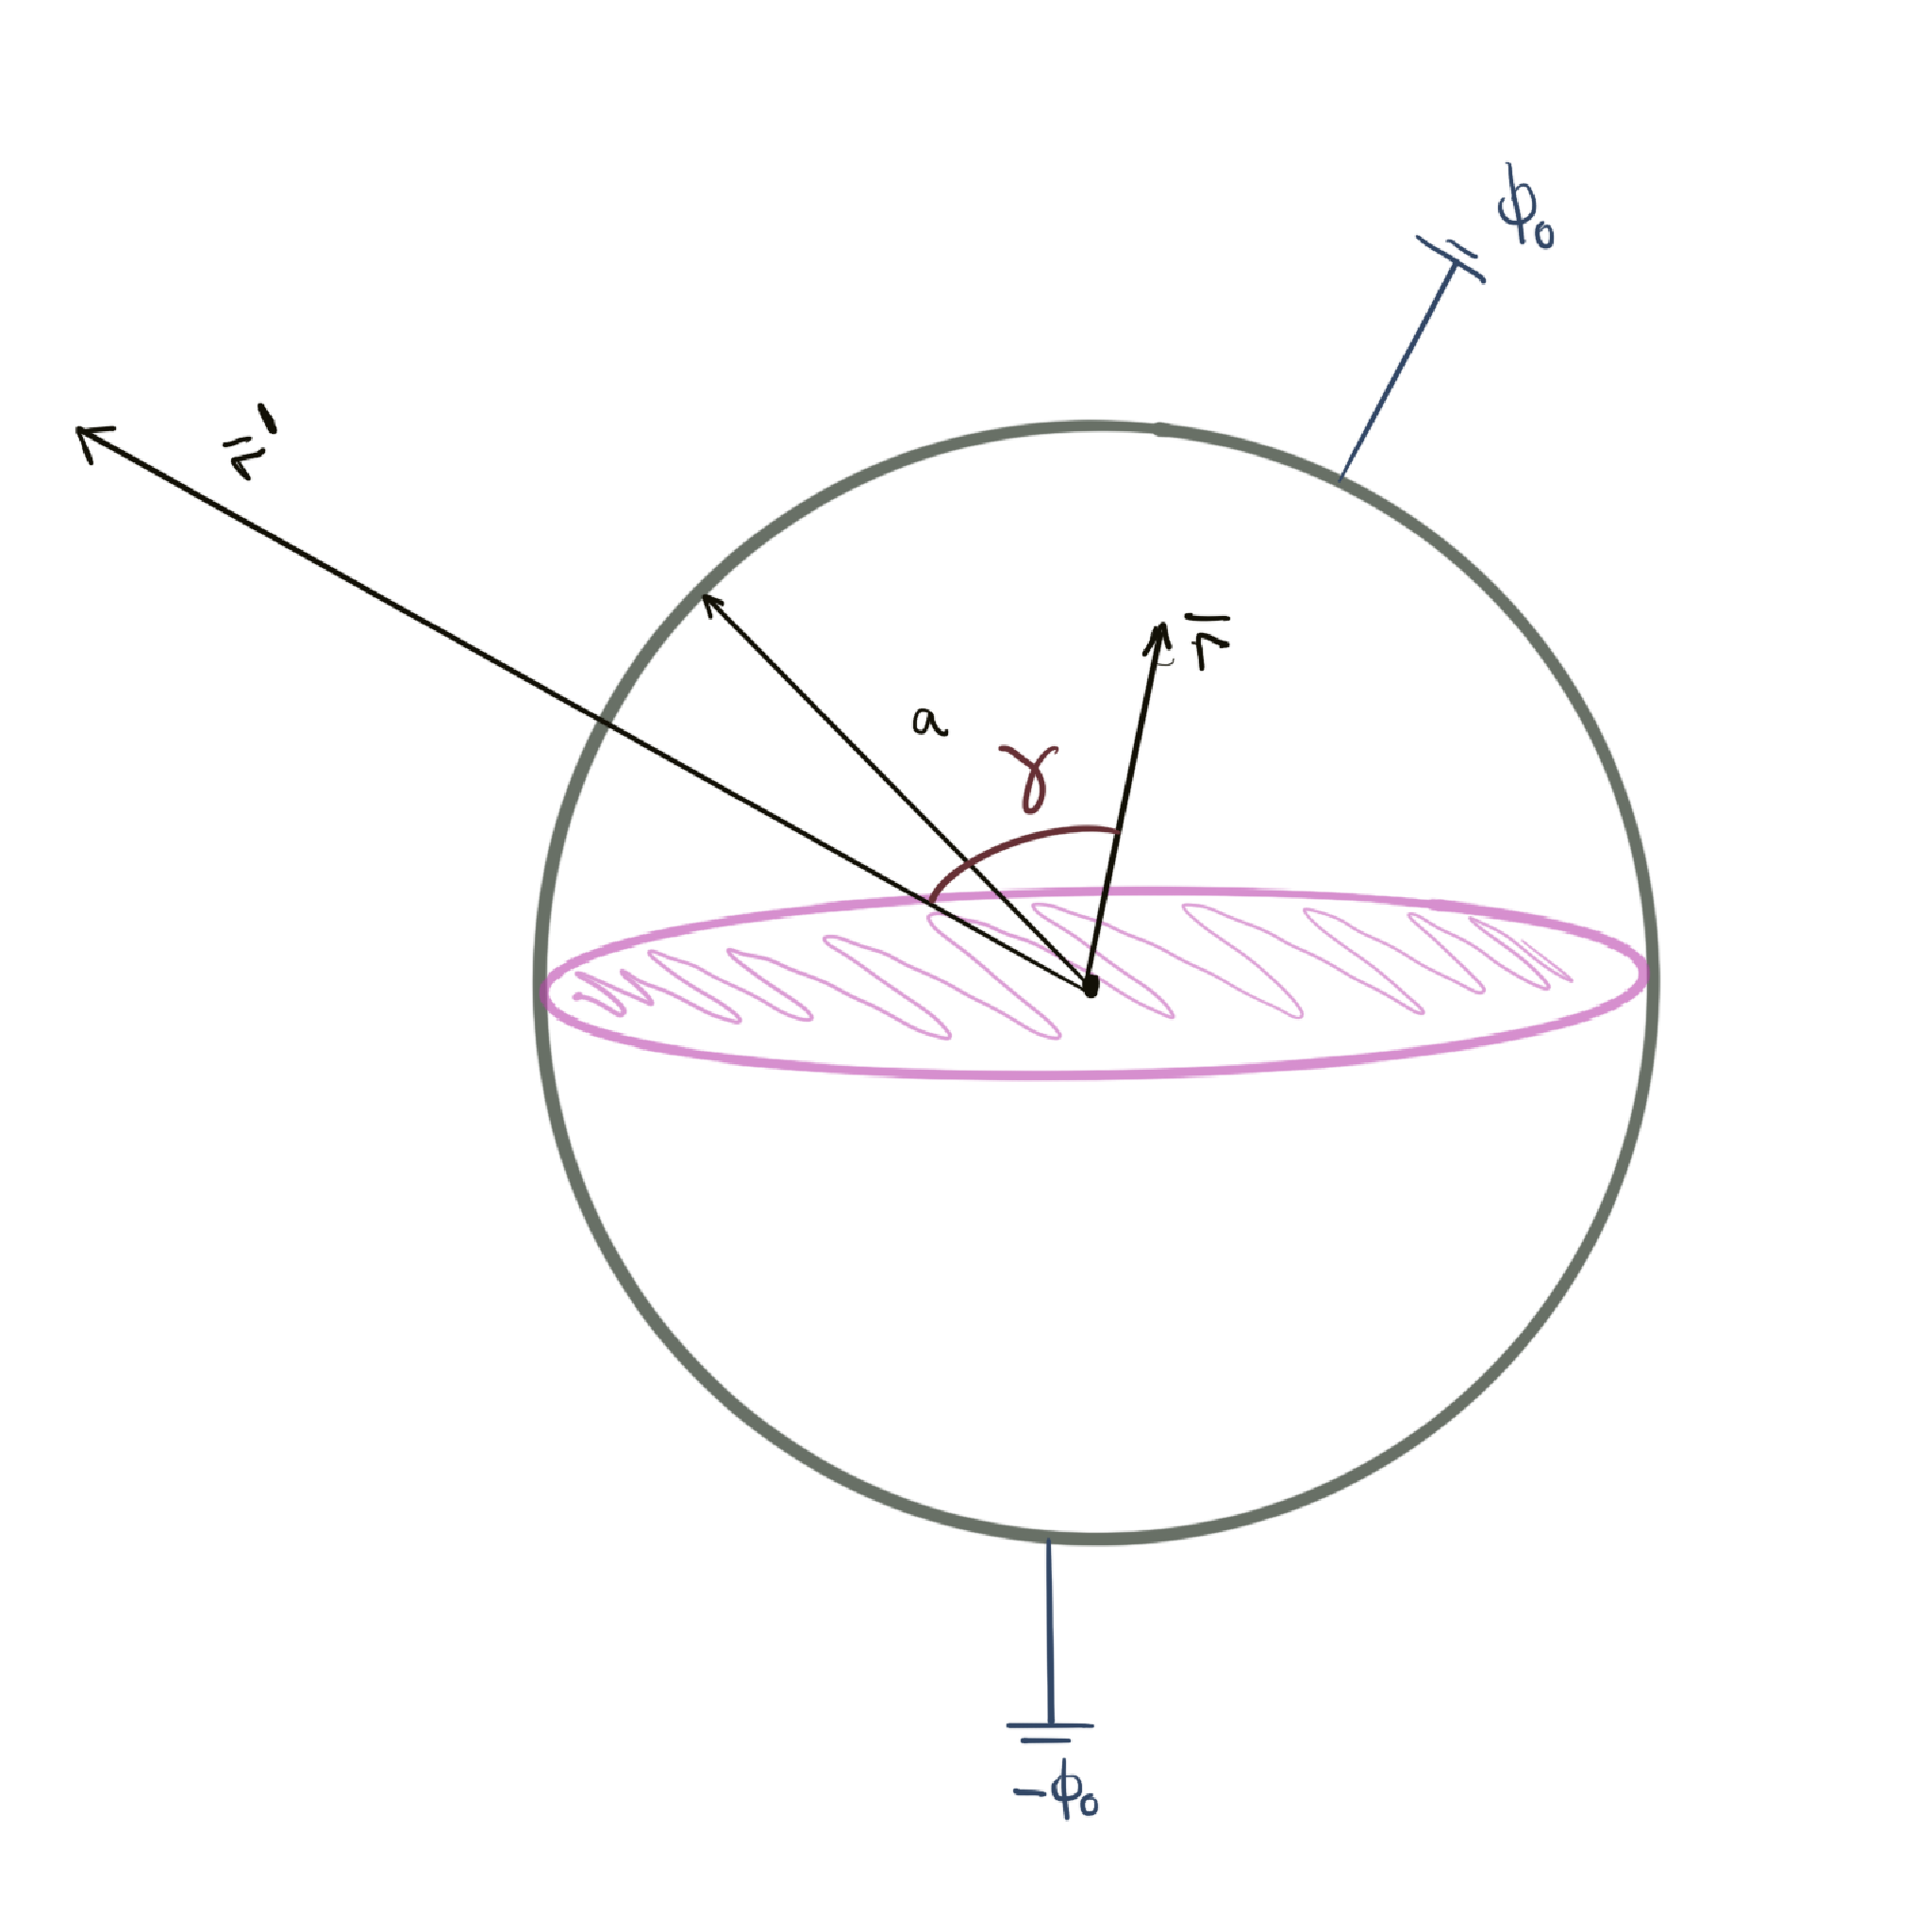
\includegraphics[width=8cm]{figures/SphericalCavity.png}
	\centering
	\caption{A rough sketch of the system we want to study....}
\end{figure}

We also know that the final appearance of the Green's function:

\begin{equation} \label{twopropagators}
	G\left(r, r^{\prime}\right)=\underbrace{\frac{1}{\left|\vec{r}-\vec{r^{\prime}}\right|}}_{G_{1}}-\underbrace{\frac{a}{r^{\prime}\left|\vec{r}-\frac{a^{2}}{r^{\prime 2}} \vec{r^{\prime}}\right|}}_{G_{2}}.
\end{equation}

So we have to basically massage two previous terms $G_{1}$ and $G_{2}$ to arrive to the desired result. Let's start by studying $G_{1}$.  We know that, by addition theorem for spherical harmonics, $G_{1}$ can be expressed as:
	
\begin{equation}\label{propagator}
	G\left(r, r^{\prime}\right) = \frac{1}{\left|\vec{r}-\vec{r^{\prime}}\right|}=4 \pi \sum_{l, m} \frac{1}{2 l+1}\frac{r_{<}^{l}}{r_{>}^{l+1}} Y_{l, m}^{*}\left(\theta^{\prime}, \phi^{\prime}\right) Y_{l, m}(\theta, \phi).
\end{equation}

So this part of the Green's function does not need more explanation. On the other hand, $G_{2}$ requires some changes before we can apply previous expression. Starting from:
	
\begin{equation}
	G_{2} (r, r^{\prime}) = -\vec{r^{\prime}}-\frac{a}{r^{\prime}\left|\vec{r}-\frac{a^{2}}{r^{\prime 2}} \vec{r^{\prime}}\right|},
\end{equation}

We can expand the norm in the denominator, put $r'$ inside the square root and extract an overall $a$ from the square root to see:
	
\begin{equation}
	G_{2} (r, r^{\prime})= \frac{-\cancel{a}}{\sqrt{\cancel{a^{2}}\left(\tfrac{(r'r)^{2}}{a^{2}} + a^{2} -2 r' r \cos \gamma\right)}},
\end{equation}

where $\gamma$ is the angle between both vectors $\vec{r}$ and $\vec{r'}$. We can see $r r'$ as a general vector and $\vec{a}$ as the vector position on the surface. If we undo square root to move back to an expression in terms of the norm, we immediately see that:
	
\begin{equation}
	G_{2} (r, r^{\prime})= \frac{-1}{\left|\tfrac{\vec{r r^{\prime}}}{a}-\vec{a}\right|}.
\end{equation}

From here, is easy to connect this expression with that of (\ref{propagator}), as they have the same form. Introducing this new term in eq (\ref{twopropagators}) we arrive to the conclusion that (massaging powers along the way):
	
\begin{equation}
	G\left(r, r^{\prime}\right)=4 \pi \sum_{l, m} \frac{1}{2 l+1}\left[\frac{r_{<}^{l}}{r_{>}^{l+1}}-\frac{1}{a}\left(\frac{a^{2}}{r r^{\prime}}\right)^{l+1}\right] Y_{l, m}^{*}\left(\theta^{\prime}, \phi^{\prime}\right) Y_{l, m}(\theta, \phi),
\end{equation}

As we wanted to show.
	
	
\textbf{2):}
	
We would like to arrive to an expression of the form:

\begin{equation}
	\Phi(r, \theta, \phi)=\sum_{l m}\frac{1}{a^{2}}\left(\frac{a}{r}\right)^{l+1} Y_{l, m}(\theta, \phi) \int \Phi_{0}\left(\theta^{\prime}, \phi^{\prime}\right) Y_{l, m}^{*}\left(\theta^{\prime}, \phi^{\prime}\right) d \Sigma^{\prime},
\end{equation}

This implies that we should start from the most general expression for a potential in terms of the Green's function, i.e:

\begin{equation}\label{generalexpresionpot}
	\Phi(r,\theta, \phi) = \frac{1}{4 \pi \epsilon_{0}} \int_{V} \rho(x')\: G(x,x') \:d^{3} x - \frac{1}{4 \pi} \oint_{S} \Phi(x') \frac{\partial G}{\partial n'} d A' .
\end{equation}

As we do not have any charge distribution in this given problem, this means $\rho(x') =0$. So the first term will not contribute. The next step, is to evaluate the interior of the remaining integral on the boundary where we can fix some parameters. In this case, the boundary condition is such that:
	
\begin{equation}
	\frac{\partial G}{\partial n'}\biggr\rvert_{n' =a}\qquad \qquad \qquad \Phi(a, \theta, \phi) = \pm \phi_{0}.
\end{equation}

Then, we have to evaluate the derivative of the Green's function $G$ with respect to the normal $n' = r'$ on the surface of the sphere (i.e $r'=a$ after derivation). After some algebra and powers manipulation, the result is:
	
\begin{equation}
	\frac{\partial G}{\partial n'}\biggr\rvert_{n' =a}=4 \pi \sum_{l, m} \frac{l+1}{2 l+1}\:\left(\frac{a^{l-1}}{r^{l+1}}\right) Y_{l, m}^{*}\left(\theta^{\prime}, \phi^{\prime}\right) Y_{l, m}(\theta, \phi).
\end{equation}

So taking this result and introducing inside expression (\ref{generalexpresionpot}), together with the boundary condition on the surface that $\Phi(a, \theta, \phi) = \pm \phi_{0}$, we obtained the final desired formula as:
	
\begin{equation}
	\Phi(r, \theta, \phi)=\sum_{l m}\frac{l+1}{a^{2} (2l+1)}\left(\frac{a}{r}\right)^{l+1} Y_{l, m}(\theta, \phi) \int \Phi_{0}\left(\theta^{\prime}, \phi^{\prime}\right) Y_{l, m}^{*}\left(\theta^{\prime}, \phi^{\prime}\right) d \Sigma^{\prime},
\end{equation}

which obviously fades out when $r\rightarrow \infty$.

\subsubsection{Green's function between concentric spheres}\label{Green's function between concentric spheres}

\textbf{1):}

First of all, we should proceed as always; To draw a sketch of the system we want to study:
	
\begin{figure}[h]
	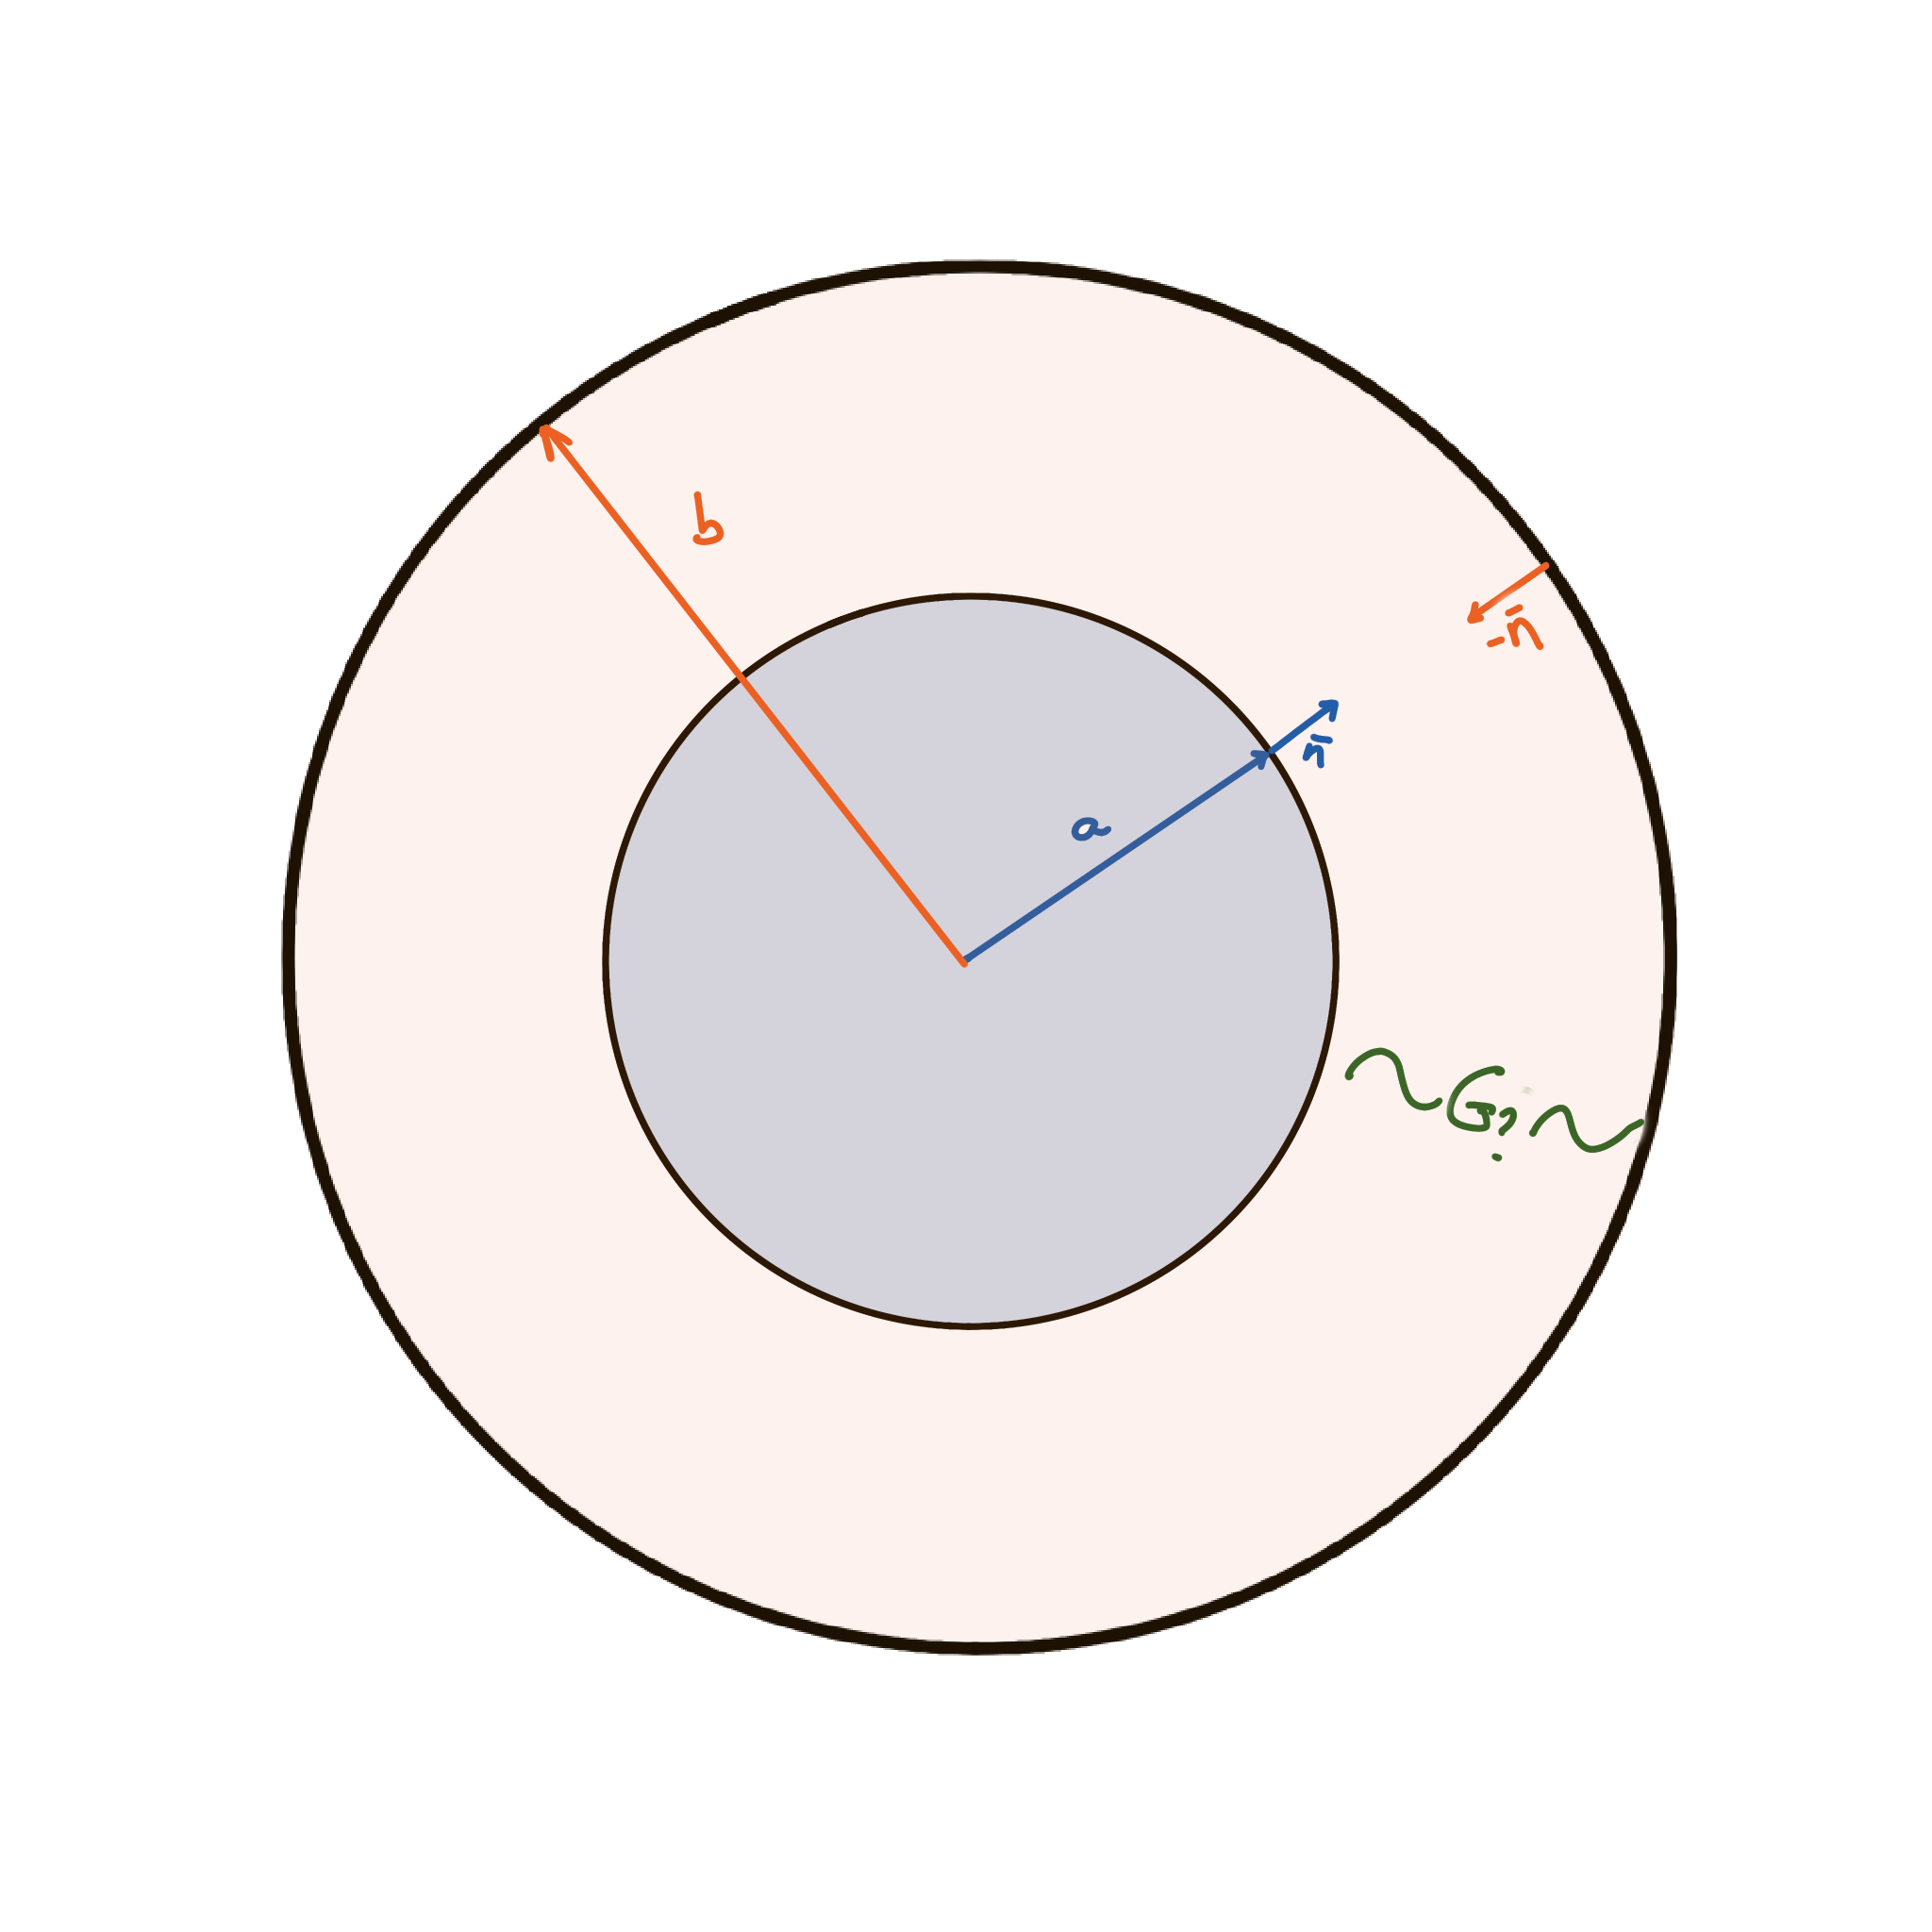
\includegraphics[width=7cm]{figures/Concentric.png}
	\centering
	\caption{Some fancy sketch of the cavity we want to study.}
\end{figure}

This first part of the problem is asking us to show that, for a given concentric spherical geometry, the radial part of the Green's function looks like:

\begin{equation}
	g_{l}\left(r, r^{\prime}\right)=\frac{r_{<}^{l}}{r_{>}^{l+1}}+\frac{1}{b^{2 l+1}-a^{2 l+1}}\left[\frac{l+1}{l}\left(r r^{\prime}\right)^{l}+\frac{l}{l+1} \frac{(a b)^{2 l+1}}{\left(r r^{\prime}\right)^{l+1}}+a^{2 l+1}\left(\frac{r^{l}}{r^{\prime l+1}}+\frac{r^{' l}}{r^{l+1}}\right)\right].
\end{equation}

With a hint stating that any Green's function can be decomposed in its radial part and its spherical part, as a linear combination of spherical harmonics of the form:

\begin{equation}\label{eq:Greenfun}
	G\left(x, x^{\prime}\right)=\sum_{l=0}^{\infty} g_{l}\left(r, r^{\prime}\right) P_{l}(\cos \gamma),
\end{equation}

Furthermore, we know that the Neumann's boundary condition states that:

\begin{equation}
	\frac{\partial}{\partial n^{\prime}} G\left(x, x^{\prime}\right)=-\frac{4 \pi}{S},
\end{equation}

So we basically have all ingredients to solve this part of the problem. If we know the boundary condition appearance for the general Green's function, we also know it for its radial part. We just have to fix the coefficients $A_{l}$ and $B_{l}$ inside $g_{l}$ making use of the double boundary condition. Double, because we have two surface where we can evaluate.\\ When evaluating on the inner sphere with radius $a$, we get:
	
\begin{equation}\label{eq:boundarycon}
		\frac{\partial G}{\partial n'}\biggr\rvert_{a} = \sum_{l} \partial_{r} g_{l}(r,r^{\prime}) P_{l}(\cos \gamma) \biggr\rvert_{a} = \frac{1}{a^{2} + b^{2}}.
\end{equation}

Where we have used that the normal is pointing outwards, so it has positive signature. It is also remarkable to realise the following; Our previous expression (\ref{eq:boundarycon}) has neither $\theta$ nor $\phi$ dependence, although there is a Legendre polynomial involved in its LHS. So this is already stating that the only set of spherical harmonics that will contribute in this problem to fix the value of the coefficients are those ones with $l=0$ (i.e $Y_{00} = \tfrac{1}{\sqrt{4 \pi}}$.) This implies that one can express the radial part of the Green's function as:

\begin{equation}\label{eq:innersphere}
		\partial_{r'} \:g_{l}\biggr\rvert_{r'=a} = \frac{-1}{a^{2} + b^{2}}\: \delta_{l,0},
\end{equation}

Now, we can do exactly the same for the outer sphere. Here there is a crucial difference; The normal to this surface, as we want to evaluate the Green's function in the region between both spheres, is pointing \textit{inwards}, so it will cary a negative sign. The same arguments we used for the inner one applies in this case too, so the result looks like:

\begin{equation}\label{eq:outersphere}
	\partial_{r'} \:g_{l}\biggr\rvert_{r'=b} = \frac{1}{a^{2} + b^{2}} \:\delta_{l,0}.
\end{equation}

Equipped with this knowledge, let's the value of the coefficients. We know that:

\begin{equation}\label{eq:radialpart}
	g_{l}\left(r, r^{\prime}\right)=\frac{r_{<}^{l}}{r_{>}^{l+1}}+f_{l}\left(r, r^{\prime}\right) = \frac{r_{l}^{l}}{r_{>}^{l+1}} + A_{l} r^{\prime l} + B_{l} r'^{ -(l+1)}.  
\end{equation}

In this specific geometry we cannot drop any of the coefficients as we have done in previous exercises. This is due to the fact that we are now dealing with things happening inside and outside two different spheres that generate the given geometry. In any case, We have two boundary conditions values two fix two different equations, so we can solve for two different variables, $A_{l}$ and $B_{l}$.  Introducing evaluated green's radial function (\ref{eq:innersphere}) and (\ref{eq:outersphere}) as RHS of derivative with respect $r$ of (\ref{eq:radialpart}), we will get two expressions as:

\begin{align}
	\frac{l\: a^{l-1}}{r^{l+1}}+\:l\: a^{l-1} A_{l} + B_{l} \frac{-(l+1)\: a^{l}}{a^{2(l+1)}} &=\frac{1}{a^{2}+ b^{2}} \delta_{l,0},\\
	\frac{-(l+1)r^{l}}{b^{l+2}}+ l\: b^{l-1} A_{l} + B_{l} \frac{-(l+1)\: b^{l}}{b^{2(l+1)}} &=\frac{-1}{a^{2}+ b^{2}} \delta_{l,0}.
\end{align}

Next step we have to perform, is just to solve for $A_{l}$ and $B_{l}$ in this coupled system of linear equations. Without loss of generality, we can set $l \neq 0$, so we get LHS of both expressions for the most general coefficients. The good part is that this simplifies RHS to 0. Solving then, one arrives to:
	
\begin{align}
	A_{l} &= \frac{1}{a^{2l+1} + b^{2l+1}} \left(\frac{(l+1)\: r^{l}}{l} - \frac{a^{2l+1}}{r^{l+1}}\right),\\
	B_{l} &= \frac{-1}{b^{2l+1} - a^{2l+1}} \left(\frac{l\: (ab)^{2l+1}}{(l+1) r^{l+1}} + r^{l} a^{2l+1}\right).
\end{align}

The last step, after all despair and suffer we have gone through, it is just to introduce these values inside expression (\ref{eq:radialpart}), massaging it a little bit to obtain:
	
\begin{equation}\label{eq:radialpart2}
	g_{l}\left(r, r^{\prime}\right)=\frac{r_{<}^{l}}{r_{>}^{l+1}}+\frac{1}{b^{2 l+1}-a^{2 l+1}}\left[\frac{l+1}{l}\left(r r^{\prime}\right)^{l}+\frac{l}{l+1} \frac{(a b)^{2 l+1}}{\left(r r^{\prime}\right)^{l+1}}+a^{2 l+1}\left(\frac{r^{l}}{r^{\prime l+1}}+\frac{r^{\prime l}}{r^{l+1}}\right)\right],
\end{equation}
	
As we wanted to show.
	
	
\textbf{2):}

From our previous result, we can then continue in order to obtain a close expression for the potential $\Phi(r,\theta,\phi)$ in all the concentric region. Furthermore, with the potential, we can compute the value of the electric field $\vec{E}$ in that geometry. Hence, our starting point will be the expression given Neumann boundary conditions is:
	
\begin{equation}
	\Phi(r,\theta, \phi) = \frac{1}{4 \pi \epsilon_{0}} \int_{V} \rho(x')\: G(x,x') \:d^{3} x + \frac{1}{4 \pi} \oint_{S} G(r,r') \frac{\partial \Phi}{\partial n'} d A' .
\end{equation}

As always, the first question we have to raise when this expression pops up is: \textit{Is there any charge in our system?} As we do not have, this implies that $\rho =0$, so the first term will not contribute and it is the second one that does. As in the previous part, the normal $n'$ is given by the radius $r'$. Then, what is $\partial_{r'} \Phi$ inside previous expression? As we know, the gradient of the potential is minus the electric field $\vec{E}$, so in this case, we get that the derivative of $\Phi$ respect to $-r'$ is just the radial component of the electric field $\vec{E}$.
	
As we want to find a close expression for the potential, let us evaluate our previous expression for $r'=b$ (You can also do it at $r'=a$, but you will get no information, as $E_{r=a} =0$). Recall the sign of the norm when computing the derivative.
	
\begin{equation}
	\begin{split}
		\Phi(r'=b, \theta, \phi) &= \frac{1}{4\pi} \oint_{S} G(r,b) \underbrace{\frac{\partial \Phi}{\partial n'}}_{-E_{r} = E_{0} \cos \theta'}  \left(\underbrace{b^{2} \sin \theta'}_{\text{jacobian}}\right) d \Omega', \\
		&= \frac{1}{4\pi} E_{0} b^{2} \oint G(r,b) \sin \theta' \cos \theta' d \Omega'.
	\end{split}
\end{equation}

Inside of previous equation, we see our Green's function evaluated at b. Recall that this function can be decomposed in its radial part, as we shown in previous section (see eq(\ref{eq:radialpart2})) and spherical harmonics. Introducing expression (\ref{eq:Greenfun}) in previous formula, and using eq(\ref{eq:radialpart2}) we obtain:
	
\begin{equation}\label{eq:almostthere}
	\Phi(b, \theta, \phi) = \frac{E_{0}b^{2}}{4\pi} \sum_{l} \frac{4\pi}{2l+1}\: g_{l}(r,b)\: \oint_{S} \sum_{m} Y_{l,m} (\Omega) \: Y^{*}_{l',m'} (\Omega') \cos \theta' \sin \theta' d\Omega'.
\end{equation}

Now we have a crucial point. A happy idea. Maria virgin, visiting us\footnote{This a rough translation of a say we have in Spanish.}, to give us a hint. We have a $\cos$ in the game. We can exploit its presence and transform it into a spherical harmonic that can help us fix the previous expression. As you may know:
	
\begin{equation}
	Y_{1,0}(\Omega') = \sqrt{\frac{3}{4 \pi}} \cos \theta'.
\end{equation}

Introducing this in expression (\ref{eq:almostthere}), and making use of spherical harmonics orthonormality, we obtain:
	
\begin{equation}
	\Phi(b, \theta, \phi) =  \sum_{l} \frac{E_{0}b^{2}}{2l+1}\: g_{l}(r,b)\: \sqrt{\frac{4\pi}{3}}\: Y_{l,m} (\Omega) \: \delta_{m,0} \delta_{l,1}. 
\end{equation}

Simplifying annoying factors and evaluating $g_{l}(r,b)$ for $l=1$, we arrive to the well deserved expression as:

\begin{equation}
	\Phi(r, \theta)=E_{0} \frac{r \cos \theta}{1-p^{3}}\left(1+\frac{a^{3}}{2 r^{3}}\right),
\end{equation}

with notation $p=\frac{a}{b}$.  We are just there. Now take this potential and derive it respect to $\theta$ and $\phi$ to compute those electric field components as:

\begin{equation}
	E_{r}(r, \theta)=-E_{0} \frac{\cos \theta}{1-p^{3}}\left(1+\frac{a^{3}}{r^{3}}\right), \quad E_{\theta}(r, \theta)=E_{0} \frac{\sin \theta}{1-p^{3}}\left(1+\frac{a^{3}}{2 r^{3}}\right), \quad E_{\phi}(r,\theta) = 0.
\end{equation}

Finally, we are done. Congratulations to us. Take a rest, you deserve it. And some chocolate and/or fancy beverage. You deserve it even more!
		



	
	
	
	
	
	
	
